\chapter{Einführung}

Mit dem vorliegenden Artikel sollen die Einsatzmöglichkeiten der seriellen Kommunikation mit Peripheriegeräten mittels \ac{spi} verdeutlicht werden.

Das \ac{spi} ist ein in den frühen 1980er Jahren von Motorola entwickeltes Bus-System mit einem „lockeren“ Standard für einen synchronen seriellen Datenbus (Synchronous Serial Port), mit dem digitale Schaltungen nach dem Master-Slave-Prinzip miteinander verbunden werden können.

\begin{figure}[h]
    \centering
    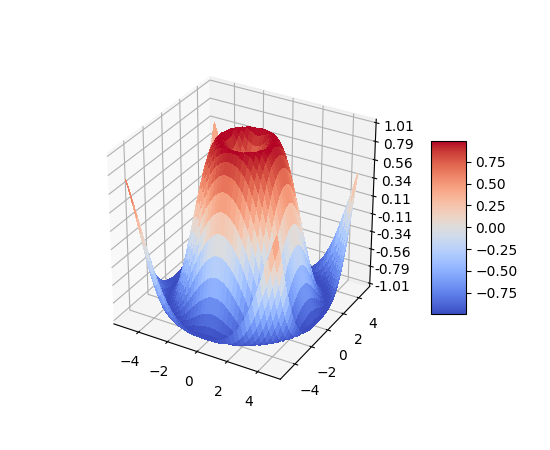
\includegraphics[width=0.25\textwidth]{surface3d_demo4}
    \caption{a nice plot}
    \label{fig:mesh1}
\end{figure}
 
As you can see in the figure \ref{fig:mesh1}, the function grows near 0. Also, in the page \pageref{fig:mesh1} is the same example.

The table \ref{table:1} is an example of referenced \LaTeX elements.
 
\begin{table}[h!]
\centering
\begin{tabular}{||c c c c||} 
 \hline
 Col1 & Col2 & Col2 & Col3 \\ [0.5ex] 
 \hline\hline
 1 & 6 & 87837 & 787 \\ 
 2 & 7 & 78 & 5415 \\
 3 & 545 & 778 & 7507 \\
 4 & 545 & 18744 & 7560 \\
 5 & 88 & 788 & 6344 \\ [1ex] 
 \hline
\end{tabular}
\caption{Table to test captions and labels}
\label{table:1}
\end{table}

\section{Aufgabenstellung}

\section{Motivation}

\section{Zielsetzung}

\section{Gliederung}